% Poster Template for the Okinawa Institute of Science and Technology (OIST)
% Created by Gaston Sivori in May 2021 based on Two-columns poster template by Jeremie Gillet (June 2019)

\documentclass[final]{beamer}

\mode<presentation>{\usetheme{OIST}}

% Packages needed for the poster
\usepackage[orientation=landscape,size=a0,scale=1.4]{beamerposter}
\usepackage[english]{babel}
\usepackage[latin1]{inputenc}

% Style of equations
\usefonttheme[onlymath]{serif}
\boldmath

% Put images in the figures folder
\graphicspath{{figures/}}

% Add packages that you need
\usepackage{amsmath}
\usepackage{lipsum}  % For dummy test
\usepackage{ragged2e} % For justifying text
\usepackage{natbib}
\usepackage[export]{adjustbox} % For vertical alignment of footer graphics

% Poster header 
\title{\huge Biologically-realistic self-supervised pattern tuning by \\somato-dendritic coupling modulation}
\author{\textbf{Gaston Sivori, Toshitake Asabuki, and Tomoki Fukai}}
\institute[OIST]{Neural Coding and Brain Computing Unit, OIST Graduate University, Okinawa, Japan}
\date[June 28th, 2021]{June 28th, 2021}

% Poster footer 
\newcommand{\leftfooter}{Okinawa Institute of Science and Technology Graduate University}
\newcommand{\rightfooter}{

\includegraphics[width=0.5in,valign=c]{tw.png} \textbf{@sivorigaston} 
\includegraphics[width=0.5in,valign=c]{email.png} \textbf{gaston.sivori@oist.jp}
}

% Poster
\begin{document}
\begin{frame}
\begin{columns}[t]

% First  column
\begin{column}{.325\textwidth}

\begin{block}{Summary}
  \justify
  \textbf{Top-down input is thought to carry both sensory and context information to basal and distal dendritic branches respectively. Bayesian inference is a strong candidate for explaining how these inputs control sensory perception. We present a biologically-plausible learning rule for dendritic synapses that reproduces the biophysical mechanisms that occur in LV cortical pyramidal (L5p) neurons. The plasticity rule maximizes the chance of coincident events by informing the synapses of the cell's output. We show that this can be achieved by simply using low-pass filtered somatic spike trains or by modeling calcium current and back-prop via somato-dendritic coupling modulation.}
\end{block}

\begin{block}{Background}
  \justify
 The coincident activation of synapses in dendritic branches of L5p cells trigger NMDA plateaus that result in broad dendritic calcium spikes. As these spikes reach the soma, repetitive neuronal firing occurs. At the same time, back-propagating action potential-activated calcium (BAC) spikes travel to the recently active dendrites inducing plasticity changes. This update mechanism would be performing a Bayesian update of the model of the input pattern (i.e., the posterior belief) through integration of local regenerative NMDA spikes \cite{larkum2009} and it should be sufficient to enable accurate and on-going perception without internally generated top-down inputs. \cite{manita2017}. The proposed model is grounded on the biophysical aspects observed in these neurons and reproduces the on-going synaptic plasticity changes that occur in active synapses by breaking apart the aspects that make such update possible. We illustrate this by informing the cell's output to the active synapses, and later, how this is achieved using calcium current as a proxy for informing the mean somatic activity as observed experimentally \cite{krieger2017}.
\end{block}

\begin{block}{Model and input scheme (Fig. 1)}
    \centering 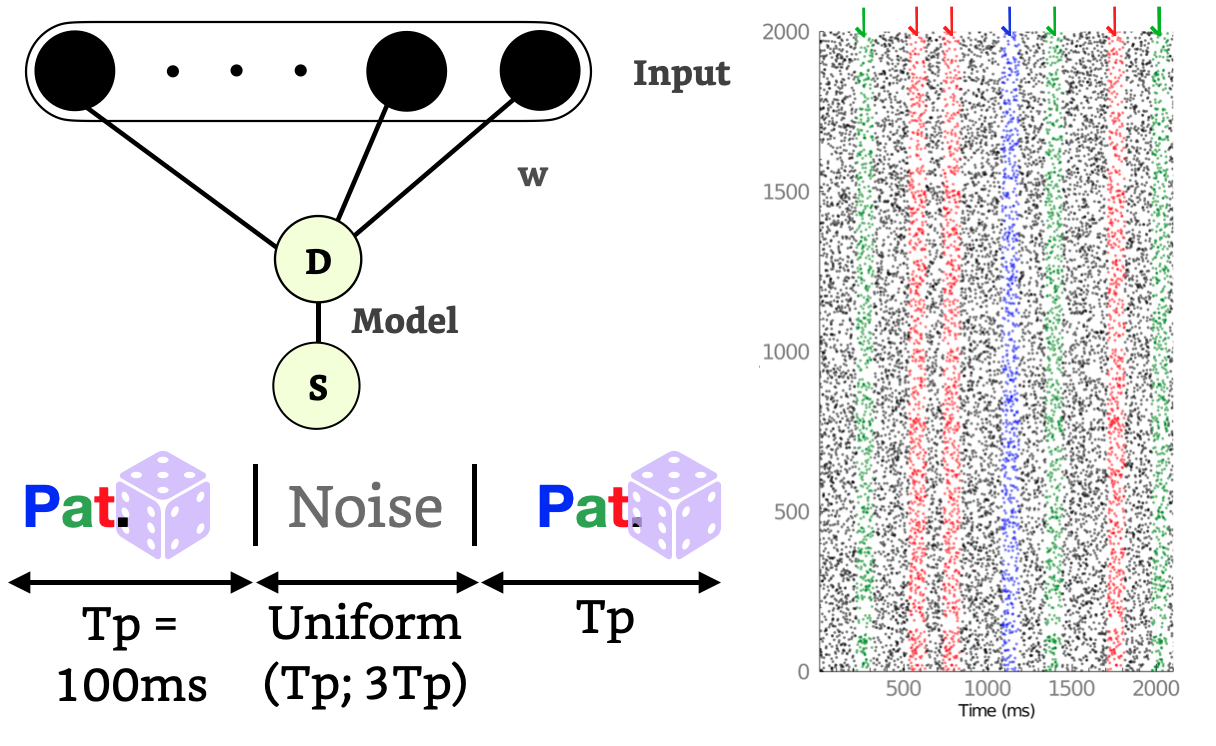
\includegraphics[width=0.9\textwidth]{fig1.png}
\end{block}
% End of first column
\end{column}

% Second column
\begin{column}{.325\textwidth}

\begin{block}{Simple LIF model (A)}
\begin{center}
\vskip-1em
  \begin{equation*}
    \mathtt{\frac{dV_{d}}{dt} = \frac{ g_{cs} (V_d - V_s) + g_e (V_E - V_d) + g_i (V_I - V_d) + g_{ld} (V_{ld} - V_d)}{C_{d}}} \nonumber
  \end{equation*}
  \begin{equation*}
    \mathtt{\frac{dV_{s}}{dt} = \frac{ g_{cd} (V_s - V_d) + g_{ls} (V_{ls} - V_s)}{C_{s}}} \nonumber
  \end{equation*}
\end{center}
  \justify
  If: $\mathtt{V_s > V_{th}}$, spike occurs. While cell is refractory, input is neglected, dendrite m.p. relaxes, and somatic m.p. resets. All synapses follow double exponential kernels (D.E.K.).
  
  \underline{\textbf{Learning rule}} \\
  With $\mathtt{Y_t}$ the somatic spike train, we impose the following plasticity induction function:
\begin{equation}
	\mathtt{PI_{i,t} = (Y_t - \frac{1}{Ti}\int_{t-Ti}^{t} Y_t \; dt) . PSP_{i,t}} \nonumber
\end{equation}
  With the main $\mathtt{PI}$ trace defined between parenthesis, $\mathtt{PI_{i,t}}$ is later low-pass filtered before inducing changes on synapses that occurred within a 5 ms time window using: $\mathtt{\tau_\Delta} \dot{\Delta_i}\mathtt{ = PI_{i,t} - \Delta_i}$ and $\dot{w_i}\mathtt{ = \eta \Delta_i}$ where $\mathtt{\tau_\Delta = 100}$ ms \cite{urbanczik2014}.
\end{block}

\begin{block}{Including calcium dynamics and $\mathtt{g_{cs}}$ modulation (B)}
  \justify
  With the same somatic compartment, we modify the dendritic compartment introducing HVA calcium channel modeled as Hodgkin-Huxley dynamics:
  \begin{equation*}
    \mathtt{Ica_t = g_{ca}m^2h(V_{ca}-V_d)} \nonumber
  \end{equation*}    
  \begin{equation*} 
    \mathtt{\tau_m} \mathtt{\frac{dm}{dt} = m_{\infty} - m} \nonumber
  \end{equation*}    
   \begin{equation*} 
    \mathtt{\tau_h} \mathtt{\frac{dh}{dt} = h_{\infty} - h} \nonumber 
  \end{equation*}
  The dynamical rates of calcium HVA channel are based on \cite{friedman1993}.

  \underline{\textbf{Revisited learning rule}} \\
  With $\mathtt{Ica_t}$ the HVA calcium dynamic trace, we impose:
\begin{equation}
	\mathtt{PI_{i,t} = (Ica_t - \frac{1}{Ti}\int_{t-Ti}^{t} Ica_t \; dt) . PSP_{i,t}} \nonumber
\end{equation}
  Similarly as above, $\mathtt{PI_{i,t}}$ is later low-pass filtered before inducing changes on synapses that occurred within 5 ms. We modulate the coupling $\mathtt{g_{cs}}$ by propagating a 60 nS pulse that occurs 1 ms during refractory period and follows D.E.K. with parameters $\mathtt{\tau_r}$ 0.5 ms and $\mathtt{\tau_d}$ 1.5 ms. Note that this model requires the upswing potential of the spike, as well as the coupling modulation, to learn.
\end{block}

\begin{block}{Remarks}
  \begin{itemize}
    \item Input consist of 2000-Poisson spike trains ($5 \pm 1$ Hz).
    \item We included synaptic transmission failure with $\mathtt{p = 0.3}$.
    \item Homeostatic plasticity is kept by scaling synapses with a factor $\kappa$ based on the totality of the absolute synaptic displacements $\mathtt{\sum |w_i|}$.
    \item Synapses are resampled from the starting Normal distribution if synaptic values exceed predefined boundaries.
  \end{itemize}
\end{block}

% End of second column
\end{column}

% Third  column
\begin{column}{.325\textwidth}

\begin{block}{Results on a sample pseudo-random seed (Figs. 2-4)}
  \justify 
  Tuning to arbitrary pattern occurs with equal probability depending on seed. \\
  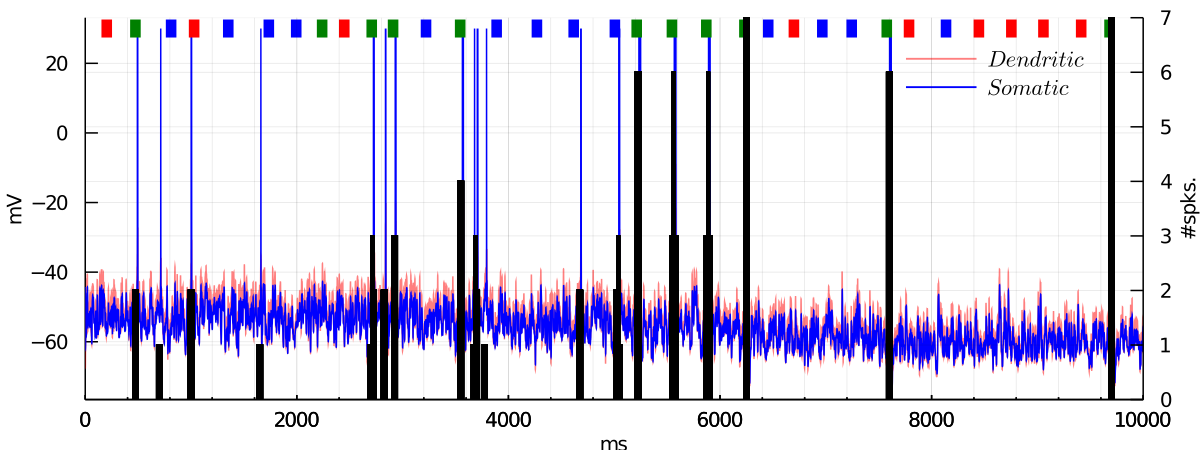
\includegraphics[width=\textwidth]{fig2.png}
  Exc. synaptic turnover is markedly higher. Distribution becomes long-tailed. \\
  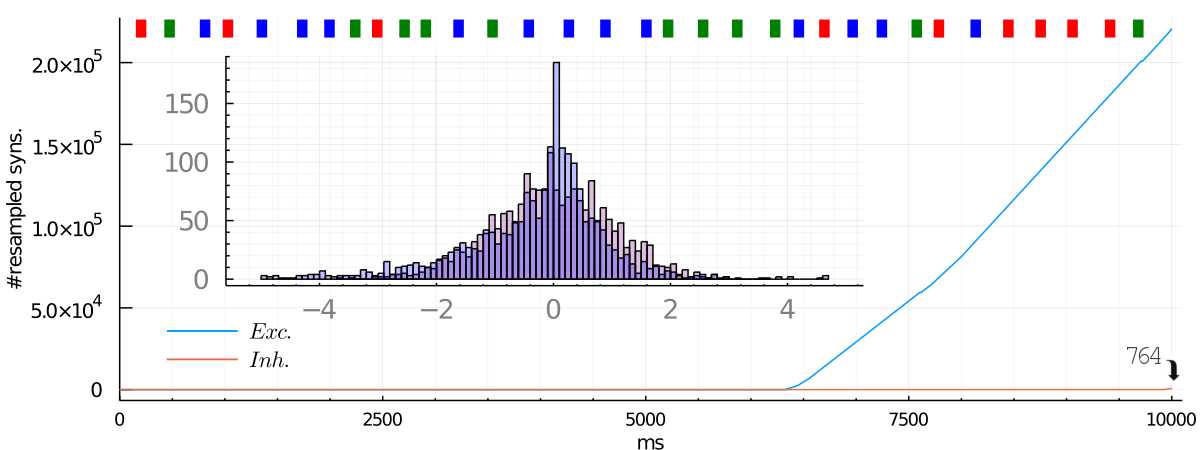
\includegraphics[width=\textwidth]{fig3.png}
  HVA channel dynamics show evidential support in PI main trace (model B). \\
  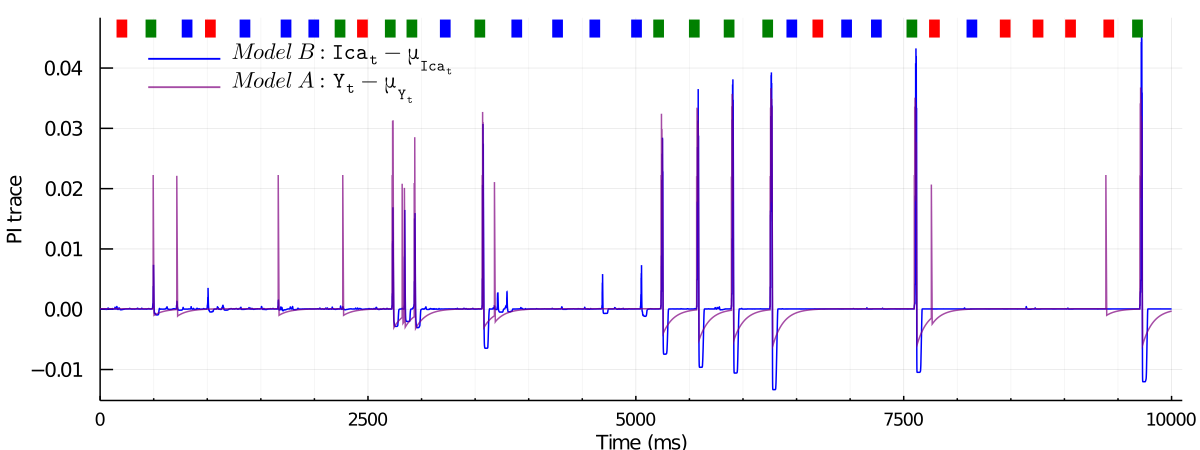
\includegraphics[width=\textwidth]{fig4.png}
  \vskip-1em
\end{block}

\begin{block}{Conclusions and future direction}
  \justify
  L5p cell dynamics are reproduced in a two-compartmental model. We will extend this into a recurrent network that is also endowed with a clustering plasticity rule.
  \vskip-1em
\end{block}

\begin{block}{References}
  \justify
    \begin{footnotesize} % Reduce the font size in this block
    \nocite{*} % Insert publications even if they are not cited in the poster
    \bibliographystyle{unsrt}
    \bibliography{Bibliography}    
    \end{footnotesize}
\end{block}
% End of third column
\end{column}

\end{columns}
\end{frame}
\end{document}
